\begin{frame}{Paradoks Einsteina, Podolsky'ego, Rosena (1935)}
Mamy dwie cząstki A i B, które oddziałują a potem zostają oddalone od siebie
\begin{itemize}
    \item Mierzymy stan najpierw cząstki A, potem B
    \item Wynik pomiaru cząstki B jest znany przed pomiarem (wnioskujemy go z A)
    \item Ale B jest daleko -- pomiar A nie mógł na nią wpłynąć
    \item Zatem zdaniem EPR wynik musiał z góry ustalony - istnieją \textit{ukryte zmienne}
\end{itemize}

\vspace{0.3em}
\pause
Wniosek EPR: Albo mechanika kwantowa jest niekompletna, albo informacja rozchodzi się
szybciej niż światło.

\end{frame}

\begin{frame}{,,Bóg nie gra w kości''}

Einstein do końca życia wierzył w lokalne zmienne ukryte --
że przyroda jest deterministyczna, a losowość w mechanice kwantowej
to tylko wyraz naszej niewiedzy.

\vspace{0.3em}
\pause
\begin{theorem}{Twierdzenie Bella (1964)}
       Jeśli istnieją ukryte zmienne to korelacje między cząstkami są ograniczone
\end{theorem}
\pause
\begin{theorem}{Nierówność CHSH ( Clauser, Horne,  Shimony, Holt 1969)}
\[
|E(a,b) + E(a,b') + E(a',b) - E(a',b')| \leq 2
\]
\end{theorem}

\end{frame}
\begin{frame}{Gra CHSH}
    \begin{figure}
        \centering
        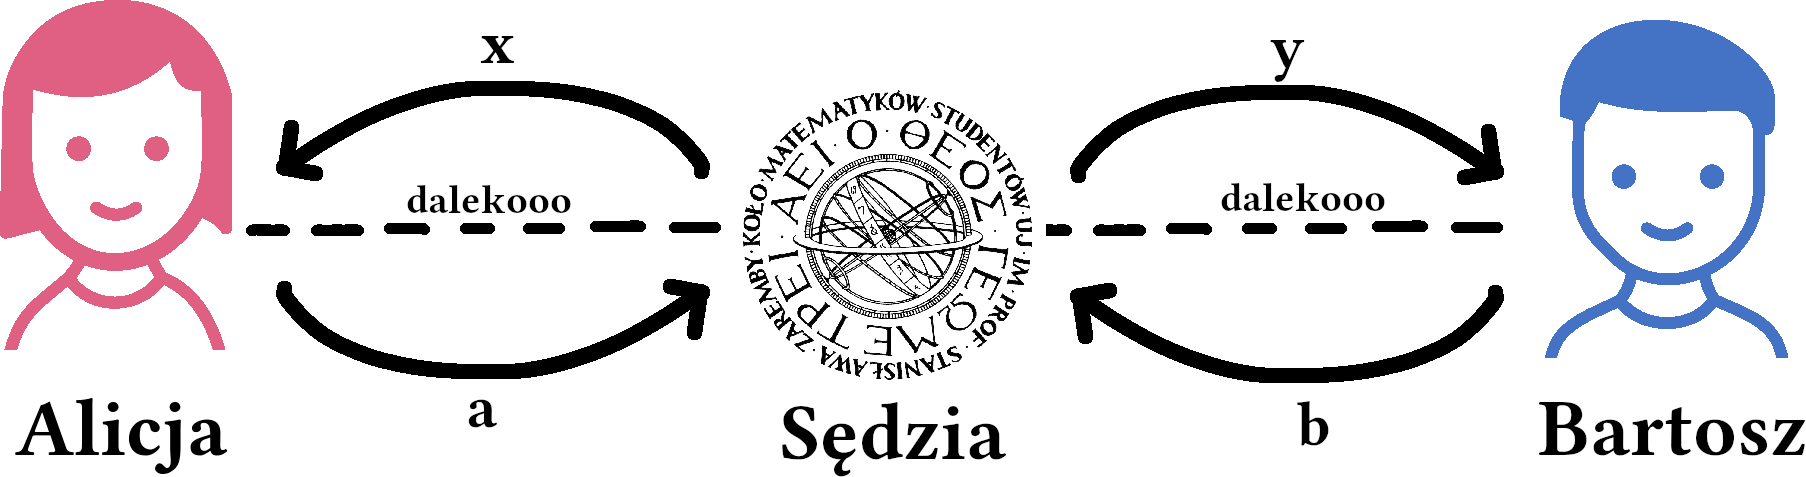
\includegraphics[width=0.65\linewidth]{images/chsh.png}
        \label{fig:enter-label}
    \end{figure}
    \begin{itemize}
        \item Sędzia losowo wybiera bity \(x\) \(y\)
        \item Wysyła bit \(x\) Alicji, bit \(y\) Bartoszowi
        \item Celem pary jest wysłanie sędziowi z powrotem takich bitów \(a\) i \(b\) aby
        \vspace{-1em}
        \[x\cdot y = a +b \mod{2}\]
        \vspace{-3em}
        \pause
        \item Gracze mogą ustalić strategię, ale NIE mogą się komunikować
    \end{itemize}
\end{frame}